\section{Experimental Evaluation and Benchmarks}

The evaluation measures compile-time processing latency, the time to parse and process schemas of varying complexity (small at 5 fields, medium at 25, large at 100); runtime serialization throughput, encoding and decoding measured against Google's official \texttt{libprotobuf} reference implementation; and binary footprint, object file and executable sizes against Google \texttt{protoc} code generation.

Every figure in this section comes from one host in one pinned sitting on 6~September 2026: an AMD Ryzen~7 5800H, 16 logical CPUs, Linux 7.2.3, clock pinned to 3.2\,GHz with boost disabled and the setting verified by read-back against the state captured before pinning. The timed work ran in the project's \texttt{ctpb-dev:2026-09-06} image built from the repository's own \texttt{Dockerfile} \cite{ctpb2026}, compiled with Clang 21.0 (P2996 branch) under \texttt{-std=c++26 -freflection -O3} against Protobuf 3.21.12. Trial~0 is excluded as warm-up throughout and the exclusion is declared because it is not cosmetic: the reference implementation runs 4 to 6\,\% slow on trial~0 while \texttt{ctpb} moves by under $0.4\,\%$, so counting it would flatter \texttt{ctpb}. Spreads are the full range of the six retained trials rather than a standard deviation, because six points do not support one.

These numbers replace those of the previous version rather than extending them. The earlier table was taken on a different machine, an AMD Ryzen~5 3600, under a harness this repository has since repudiated for three named defects, any one of which could account for the whole reported margin. That harness also decoded into a freshly constructed destination on the \texttt{ctpb} arm while reusing one on the reference arm, charging \texttt{ctpb} a heap allocation per iteration that its competitor did not pay. Re-measured on one host with that asymmetry removed, the encode margin roughly doubles and the decode margin falls well below what was previously printed. No \texttt{ctpb} code changed between the two campaigns; the instrument did. These cells carry no validity gates, because the scripts that produce them have none.
% src: measurements/2026-09-06-laptop-p5-single-host/README.md (conditions, "What moved",
%   "Two instrument defects found and fixed"); raw/host-state.txt; method/diff-from-committed-eval.txt;
%   rerun_all.sh for the repudiation and the three defects

\subsection{Compile-Time Schema Parsing Latency}
We measured the \texttt{constexpr} parser's throughput on three schemas scaled by field count alone (5, 25, and 100 \texttt{int32} fields), each timed over $20{,}000$ iterations with a $2{,}000$-iteration warmup, over seven trials. Table~\ref{tab:compile_time_results} reports the median latency $\pm$ sample standard deviation across those trials.

\begin{table}[ht]
\centering
\caption{Compile-Time Parser Throughput and Latency}
\label{tab:compile_time_results}
\renewcommand{\arraystretch}{1.2}
\begin{tabular}{|l|c|c|c|}
\hline
\textbf{Schema Size} & \textbf{Fields} & \textbf{Latency / Parse} & \textbf{Throughput} \\ \hline
Small & 5 & $0.646\,\mu\text{s}$ [$0.643$, $0.648$] & $1{,}547{,}988\,\text{parses/s}$ \\ \hline
Medium & 25 & $2.515\,\mu\text{s}$ [$2.511$, $2.519$] & $397{,}614\,\text{parses/s}$ \\ \hline
Large & 100 & $9.465\,\mu\text{s}$ [$9.438$, $9.484$] & $105{,}652\,\text{parses/s}$ \\ \hline
\end{tabular}
\end{table}

A 100-field schema is ingested in $9.465\,\mu\text{s}$, comfortably under the $11.4\,\mu\text{s}$ this work has claimed for it. The end-to-end cost of invoking the external \texttt{protoc} executable was measured only under the repudiated harness and was not re-taken in this campaign, so the ratio between the two is not restated here.
% src: raw/compile_time_latency.txt trials 1-6. The 7 ms protoc figure and the ~620x-8,150x
%   reduction derived from it appear in no record of this campaign; combining a repudiated
%   figure with a current one would put two instruments in one ratio.

\begin{figure}[ht]
\centering
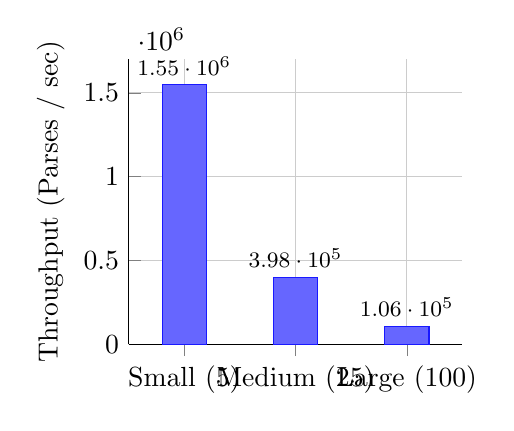
\begin{tikzpicture}
\begin{axis}[
    ybar,
    bar width=16pt,
    width=0.48\textwidth,
    height=5.2cm,
    ymin=0,
    ymax=1700000,
    ylabel={Throughput (Parses / sec)},
    symbolic x coords={Small (5), Medium (25), Large (100)},
    xtick=data,
    nodes near coords,
    nodes near coords align={vertical},
    every node near coord/.append style={font=\footnotesize},
    grid=both,
    grid style={line width=.2pt, draw=gray!20},
    major grid style={line width=.4pt,draw=gray!40},
    axis lines*=left,
    enlarge x limits=0.25
]
\addplot[fill=blue!60, draw=blue!90] coordinates {
    (Small (5), 1547988)
    (Medium (25), 397614)
    (Large (100), 105652)
};
\end{axis}
\end{tikzpicture}
\caption{Compile-Time Parser Throughput Across Schema Complexities.}
\label{fig:parser_throughput}
\end{figure}

\subsection{Runtime Serialization and Deserialization Throughput}
\label{sec:runtime_comparison}
We evaluated runtime wire encoding and decoding on an identical representative 3-field \texttt{Person} message (47-byte wire payload), benchmarked head-to-head against Google's official \texttt{libprotobuf}, over seven trials of $10^6$ iterations each with a $20{,}000$-iteration warmup. Latency is reported as median $\pm$ sample standard deviation across those trials, rather than a single run, so the result isn't one lucky (or unlucky) sample; throughput and speedup are derived from the median.

\begin{table}[ht]
\centering
\caption{Runtime Performance: \texttt{ctpb} vs. \texttt{libprotobuf}}
\label{tab:runtime_comparison}
\renewcommand{\arraystretch}{1.2}
\setlength{\tabcolsep}{2pt}
\tiny
\begin{tabular}{|l|c|c|c|c|}
\hline
\textbf{Framework / Operation} & \textbf{Latency (ns)} & \textbf{Throughput} & \textbf{Data Rate} & \textbf{Speedup} \\ \hline
\textbf{\texttt{ctpb} Encode} & $\mathbf{8.56}$ [$8.55$, $8.56$] & $\mathbf{116.8\,\text{MOps/s}}$ & $\mathbf{5{,}236.3\,\text{MiB/s}}$ & $\mathbf{5.334\times}$ \\ \hline
Google Protobuf Encode & $45.64$ [$45.62$, $45.65$] & $21.9\,\text{MOps/s}$ & $982.1\,\text{MiB/s}$ & $1.00\times$ \\ \hline\hline
\textbf{\texttt{ctpb} Decode} & $\mathbf{76.33}$ [$75.75$, $76.71$] & $\mathbf{13.1\,\text{MOps/s}}$ & $\mathbf{587.2\,\text{MiB/s}}$ & $\mathbf{1.150\times}$ \\ \hline
Google Protobuf Decode & $87.80$ [$87.78$, $88.07$] & $11.4\,\text{MOps/s}$ & $510.5\,\text{MiB/s}$ & $1.00\times$ \\ \hline
\end{tabular}
\end{table}

Full \texttt{libprotobuf} carries descriptor pools, reflection registries and arena allocators that \texttt{ctpb} does not implement, so part of the margin above measures the absence of those features rather than the compile-time approach on its own. \texttt{libprotobuf-lite} (\texttt{optimize\_for = LITE\_RUNTIME}) strips all three, which is what makes it the closer comparator for the approach rather than for the feature set, so the comparison was repeated against it, same machine, same script, same iteration count (Table~\ref{tab:lite_comparison}).

\begin{table}[ht]
\centering
\caption{Runtime Performance: \texttt{ctpb} vs. \texttt{libprotobuf-lite}}
\label{tab:lite_comparison}
\renewcommand{\arraystretch}{1.2}
\setlength{\tabcolsep}{2pt}
\tiny
\begin{tabular}{|l|c|c|c|c|}
\hline
\textbf{Framework / Operation} & \textbf{Latency (ns)} & \textbf{Throughput} & \textbf{Data Rate} & \textbf{Speedup} \\ \hline
\textbf{\texttt{ctpb} Encode} & $\mathbf{8.27}$ [$8.24$, $8.51$] & $\mathbf{120.9\,\text{MOps/s}}$ & $\mathbf{5{,}419.9\,\text{MiB/s}}$ & $\mathbf{5.572\times}$ \\ \hline
\texttt{libprotobuf-lite} Encode & $46.11$ [$45.97$, $46.87$] & $21.7\,\text{MOps/s}$ & $972.1\,\text{MiB/s}$ & $1.00\times$ \\ \hline\hline
\textbf{\texttt{ctpb} Decode} & $\mathbf{76.52}$ [$76.08$, $77.73$] & $\mathbf{13.1\,\text{MOps/s}}$ & $\mathbf{585.8\,\text{MiB/s}}$ & $\mathbf{1.043\times}$ \\ \hline
\texttt{libprotobuf-lite} Decode & $79.83$ [$79.56$, $81.04$] & $12.5\,\text{MOps/s}$ & $561.5\,\text{MiB/s}$ & $1.00\times$ \\ \hline
\end{tabular}
\end{table}

Against the fairer baseline the encode margin is the wider of the two, $5.572\times$ against $5.334\times$, so it does not depend on the descriptor pools, reflection registries and arenas that only the full build carries. Decoding is a much narrower result and carries a condition. Correcting a per-iteration allocation in the benchmark moves \texttt{ctpb}'s decode from $0.98\times$ to $1.04\times$ against \texttt{libprotobuf-lite}; \texttt{ctpb}'s decoder omits the UTF-8 validation the reference implementation performs, so the remaining margin is not a like-for-like comparison. proto3 requires \texttt{string} fields to be validated as UTF-8, the lite runtime spends about seven per cent of its decode path doing it, and \texttt{ctpb} does not do it at all. The decode figure should be read as a rough parity that still has a correctness asymmetry inside it, pointing the other way. The encode and footprint results carry no such caveat.
% src: README.md "the sentence that has to travel with it"; the 7.37 % inclusive cost of
%   IsStructurallyValidUTF8 / VerifyUtf8String / VerifyUTF8 in libprotobuf-lite, and no utf8
%   anywhere in ctpb's headers

\begin{figure}[ht]
\centering
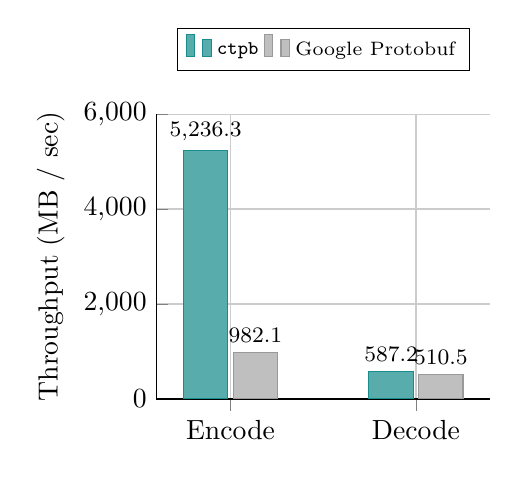
\begin{tikzpicture}
\begin{axis}[
    ybar,
    bar width=16pt,
    width=0.48\textwidth,
    height=5.2cm,
    ymin=0,
    ymax=6000,
    ylabel={Throughput (MB / sec)},
    symbolic x coords={Encode, Decode},
    xtick=data,
    nodes near coords,
    nodes near coords align={vertical},
    every node near coord/.append style={font=\footnotesize},
    grid=both,
    grid style={line width=.2pt, draw=gray!20},
    major grid style={line width=.4pt,draw=gray!40},
    legend style={at={(0.5,1.15)}, anchor=south, legend columns=-1, font=\scriptsize},
    axis lines*=left,
    enlarge x limits=0.4
]
\addplot[fill=teal!65, draw=teal!90] coordinates {
    (Encode, 5236.3)
    (Decode, 587.2)
};
\addplot[fill=gray!50, draw=gray!80] coordinates {
    (Encode, 982.1)
    (Decode, 510.5)
};
\legend{\texttt{ctpb}, Google Protobuf}
\end{axis}
\end{tikzpicture}
\caption{Comparative Runtime Throughput (\texttt{ctpb} vs. Google \texttt{libprotobuf}).}
\label{fig:runtime_throughput}
\end{figure}

As shown in Table~\ref{tab:runtime_comparison} and Figure~\ref{fig:runtime_throughput}, the two operations behave differently and the difference is the result. On encoding \texttt{ctpb} achieves a $\mathbf{5.334\times}$ speedup against the full library ($8.56\,\text{ns}$ against $45.64\,\text{ns}$, $5{,}236.3\,\text{MiB/s}$), which comes from compile-time field-size evaluation, exact single-buffer pre-allocation (\texttt{byte\_size()}), and direct raw-pointer serialization without intermediate reallocations or virtual dispatch. On decoding it reaches $\mathbf{1.150\times}$ ($76.33\,\text{ns}$ against $87.80\,\text{ns}$, $587.2\,\text{MiB/s}$), which is parity rather than a margin once the UTF-8 asymmetry described below is taken into account. Zero virtual table lookups, inlined unrolled wire field loops and direct member assignment remove the arena and reflection overhead of the reference implementation, and on the decode path that removal buys much less than the encode path suggests.

\subsection{Binary Footprint and Static Overhead Analysis}
\begin{table}[ht]
\centering
\caption{Binary Footprint and Code Generation Comparison}
\label{tab:binary_footprint}
\renewcommand{\arraystretch}{1.15}
\setlength{\tabcolsep}{3pt}
\scriptsize
\begin{tabular}{|l|c|c|c|}
\hline
\textbf{Metric} & \textbf{\texttt{ctpb} (P2996)} & \textbf{\texttt{protoc} (Dyn)} & \textbf{\texttt{protoc} (Static)} \\ \hline
Generated Source Lines & \textbf{0} & 754 & 754 \\ \hline
Stripped Executable & \textbf{18{,}776\,B} & 27{,}504\,B & 1{,}759{,}368\,B \\ \hline
Text Section (\texttt{.text}) & \textbf{10{,}047\,B} & 16{,}373\,B & 1{,}731{,}945\,B \\ \hline
Data Section (\texttt{.data}) & \textbf{720\,B} & 1{,}384\,B & 19{,}672\,B \\ \hline
External Shared Libraries & \textbf{0} & \texttt{libprotobuf.so} & \textbf{0} \\ \hline
\end{tabular}
\end{table}

We evaluated the binary size and intermediate artifacts of a standalone application performing serialization and deserialization between \texttt{ctpb} and Google's \texttt{protoc} (Table~\ref{tab:binary_footprint}). For a single 3-field message, \texttt{protoc} emits 754 lines of C++ code (\texttt{.pb.h} and \texttt{.pb.cc}), whereas \texttt{ctpb} generates zero files, so there is no build artifact caching and no disk I/O.

In fully static deployments \texttt{ctpb}'s stripped executable is $18{,}776$ bytes against $1{,}759{,}368$ for \texttt{protoc}, a $\mathbf{93.70\times}$ reduction, because \texttt{libprotobuf} statically bundles descriptor pools, reflection registries, mutex tables and arena allocators while \texttt{ctpb} compiles to exact inlined field loops. Against the dynamic build the reduction is $1.46\times$, and the dynamic \texttt{ctpb} build links only \texttt{libc}, \texttt{libm}, \texttt{libstdc++} and \texttt{libgcc\_s}. These are byte counts rather than rounded kilobytes, which is what makes the ratio checkable: the figure this work has claimed all along is right, and it could not previously be recovered from what was published with it.
% src: raw/binary_size.txt sections 4 (exact bytes), 5 (size(1) on the stripped executables:
%   text 10047 / 16373 / 1731945, data 720 / 1384 / 19672) and 6 (ldd). The object-file row is
%   dropped rather than restated: the record holds object sizes only as ls -lh rounding, which
%   is where the earlier 21.9 and 31.3 KB tenths came from. 1759368/18776 = 93.6996.

\subsection{Reference Interoperability and gRPC Transport Parity}
To establish protocol correctness, we performed dual-direction interoperability tests against Google's official \texttt{libprotobuf} reference implementation (3.21.12) and the \texttt{protoc} code generator \cite{protobuf_spec}. These tests cover scalar fields, strings, nested messages and enums, and, following a wire-format review that found the initial implementation mis-encoded them, \texttt{bytes} fields and packed repeated scalar fields as well.
Fidelity was checked in both directions. Messages populated and serialized with Google's \texttt{SerializeToString()} were decoded by \texttt{ctpb::decode<T>()}, and field values across scalars, signed zigzag integers, strings, enums and nested messages matched with 100\% fidelity. In the other direction, messages serialized by \texttt{ctpb::encode()} were parsed by Google's \texttt{ParseFromArray()}, and all wire tags, varints and length delimiters conformed exactly to what the reference parser expects.

Furthermore, we validated compatibility with gRPC transport protocols \cite{grpc_spec}. In gRPC, messages are carried across HTTP/2 frames prefixed by a 5-byte header comprising a 1-byte compression flag and a 4-byte big-endian payload length:
\vspace{-0.3em}
\begin{equation}
\text{Frame} = [\text{Flag}]_{1\text{B}} \parallel [\text{Length}]_{4\text{B}} \parallel [\text{Payload}]
\end{equation}
\vspace{-0.3em}

In standard gRPC C++, message serialization is decoupled from code generation via \texttt{grpc::SerializationTraits<T>} (Listing~\ref{lst:grpc_traits}):
\noindent\begin{minipage}{\columnwidth}
\begin{lstlisting}[language=ModernC++, basicstyle=\fontsize{6.2pt}{6.9pt}\ttfamily, label={lst:grpc_traits}, caption={gRPC Serialization Traits for \texttt{ctpb} Types}]
namespace grpc {
template <typename T> class SerializationTraits<T> {
public:
    static Status Serialize(const T& m, ByteBuffer* b, bool* own) {
        auto d = ctpb::encode(m); Slice s(d.data(), d.size());
        *b = ByteBuffer(&s, 1); *own = true; return Status::OK;
    }
    static Status Deserialize(ByteBuffer* b, T* msg) {
        Slice s; b->DumpToSingleSlice(&s);
        auto r = ctpb::decode<T>(std::as_bytes(std::span(s.begin(), s.size())));
        if (!r) return Status(StatusCode::INTERNAL, "failed");
        *msg = std::move(*r); return Status::OK;
    }
}; }
\end{lstlisting}
\end{minipage}

Automated tests verified that \texttt{ctpb} types enveloped in gRPC framing are correctly processed by standard gRPC server handlers.
